\section{결합 방법: 상위 불변 + 코드 어댑터}
\label{sec:coupling}

두 모듈이 각자 최대 성능을 내도, 명령 형식의 어긋남, 좌표 변환의 차이, 지연, 서로 본 적 없는 입력 분포 때문에 연결에서 성능이 샐 수 있다. 앞선 두 층 구현에서는 VLA 단독 \tentative{12}편 중 \tentative{8}편이 모델이 아니라 층 사이 런타임의 멈춤 고리로 끝났다(\cref{sec:evidence}). 결합은 상위 VLM을 건드리지 않는 것을 최우선으로 한다: 상위는 지금 학습한 형식·성능 그대로 두고, 인터페이스의 모든 변환과 조종 방식은 규칙 코드 어댑터가 맡는다. 그래서 결합은 어댑터·타이밍·학습의 세 겹으로 설계하고, 새는 양을 연결 손실로 직접 잰다.

\subsection{인터페이스: 코드 어댑터}
\label{sec:adapter}
상위 출력 형식은 지금 학습 그대로다: 목표 점(영상 좌표), 높이 의도, 그리퍼 의도, 진행 평가. 새 출력을 추가하지 않고 재학습도 하지 않는다. 코드 어댑터(규칙, 학습 없음)가 이 네 가지를 JCR 명령으로 바꾼다.
\begin{itemize}
  \item \textbf{목적지 xyz:} 목표 점을 공용 코드가 센서 깊이로 바꾼다(상위와 JCR가 같은 코드를 공유, \cref{sec:upper}).
  \item \textbf{대상 물체 마스크:} 목표 점 둘레를 머리·손목 영상에 표시해 JCR에게 어떤 물체를 다루는지 준다.
  \item \textbf{단계:} 높이 의도를 그대로 옮긴다(이동·근접·잡기/놓기).
  \item \textbf{그리퍼 허용:} 그리퍼 의도를 이진값으로 옮긴다.
  \item \textbf{끌림 세기:} 단계별 규칙값 $\kappa$(운반 중 0.3, 먼 접근 0.5, 잡기·놓기 높이이거나 목적지 5\,cm 안이면 0.9). 딱딱한 허용 범위로 자르는 대신 끌림으로 조종하고, 넓은 안전 범위(10\,cm)만 자름으로 강제한다(\cref{sec:vla}).
  \item \textbf{명령 나이:} 명령이 나온 뒤 지난 시간.
\end{itemize}
JCR 보고(접촉, 잡기 성공, 이상 신호)는 어댑터가 문장으로 바꿔 상위의 기존 `직전 명령과 결과' 입력 칸에 넣는다(\cref{fig:upper}) — 상위 입력 형식도 바뀌지 않는다. 픽셀$\rightarrow$xyz 변환과 카메라 보정은 상위와 JCR가 함께 쓰는 공용 코드 하나로 두고, 왕복 변환 단위 시험으로 고정한다. 1단계와 2단계는 같은 어댑터와 같은 변환 코드를 쓴다.

\subsection{타이밍: 도착 뒤 재질의, JCR가 이어감}
\label{sec:timing}

\begin{figure*}[t]
\centering
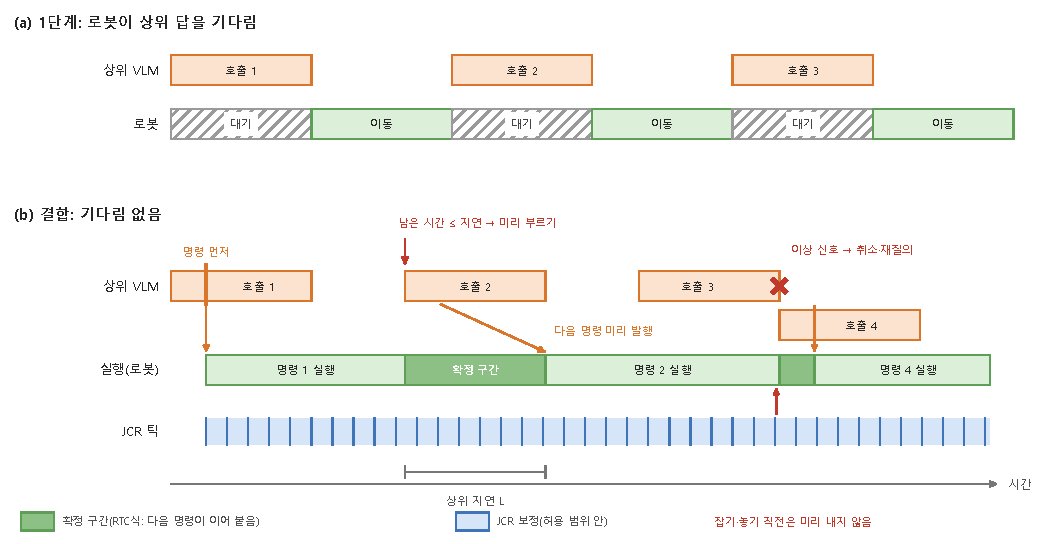
\includegraphics[width=\linewidth]{figures/f4_timeline.pdf}
\caption{\textbf{결합 시간축(개념도, 시간 눈금 없음).} (a) 1단계: 로봇은 상위가 답하는 동안 기다린다. (b) 결합: 재질의는 도착 뒤, 곧 상위가 학습한 장면 그대로다. 상위가 1--3\,s 생각하는 동안 JCR는 끌림을 따라 정렬·잡기·들기 시작을 이어가 로봇이 멈추지 않는다. 이상 신호가 오면 도착 전이라도 취소하고 다시 묻는다. 도착 전 미리 부르기(점선, 선택)는 상위 추가 학습이 필요한 나중 확장이다.}
\label{fig:timeline}
\end{figure*}

명령 먼저 출력과 도착 뒤 재질의 두 가지를 함께 쓴다(\cref{fig:timeline}).
\begin{enumerate}
  \item \textbf{명령 먼저 출력:} 상위 답의 맨 앞에 명령을 두고, 명령 부분이 생성되는 즉시 어댑터를 거쳐 실행한다. 고정 프롬프트는 캐시한다. 호출당 첫 명령까지의 시간을 잰다.
  \item \textbf{도착 뒤 재질의, 생각하는 동안 JCR가 이어감:} 상위를 다시 부르는 시점은 도착 뒤로 고정한다 — 상위가 학습 때 본 장면(1단계의 `도착·검증'과 같은 상황)을 그대로 준다. 호출에 걸리는 1--3\,s(측정한 호출 지연) 동안 로봇을 세워 두지 않고, 어댑터가 JCR에 작은 이어가기 명령을 준다: 잡기 성공 뒤에는 들기 시작 +3\,cm, 놓은 뒤에는 +2\,cm 물러나기다. 예상 밖 접촉·대상 이동 등 이상 신호가 오면 도착 전이라도 취소하고 즉시 다시 묻는다.
\end{enumerate}
평가는 판당 대기 시간, 성공률, 취소율을 함께 보며, 연결 손실이 나빠지지 않아야 채택한다.

\paragraph{(선택) 확장: 도착 전 미리 부르기.} 사건 기준 미리 부르기~\cite{eventtrig2026}와 RTC식 겹치기~\cite{black2025rtc}로 상위가 도착 전에 다음 명령을 미리 내게 할 수 있지만, 이는 상위가 아직 학습하지 않은 입력(도착 예상 표시)과 출력(미리 내도 되나 표지)을 요구해 상위 추가 학습이 필요하다. 지금은 선발행 확률 $p_{\text{pre}} = 0$으로 꺼 두고, 상위 성능을 유지한 채로 결합이 먼저 되는지 본 뒤의 나중 선택지로 둔다(\cref{sec:mesh}).

\subsection{학습: 상위는 동결, JCR만 어댑터 명령으로}
\label{sec:mesh}

\begin{figure*}[t]
\centering
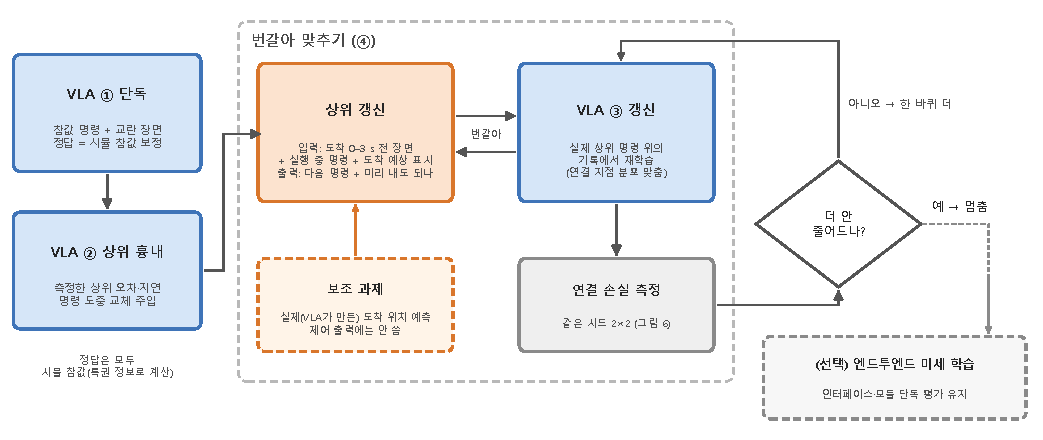
\includegraphics[width=\linewidth]{figures/f5_training.pdf}
\caption{\textbf{결합 학습 루프.} 상위는 지금 학습한 체크포인트로 동결한다. JCR는 단독(①)과 상위 오차 흉내(②)로 시작해, 동결한 상위 + 코드 어댑터를 붙여 돈 실제 기록에서 다시 학습하고(③), 라운드마다 반복 정착한다(④, JCR만 갱신). 매 바퀴 같은 시드 2$\times$2로 연결 손실을 잰다. 더 줄지 않으면 멈춘다. 엔드투엔드 미세 학습과 상위 미리 내기 학습은 그 뒤의 선택지다.}
\label{fig:train}
\end{figure*}

상위 VLM을 건드리지 않는 것이 최우선이므로, 결합 학습은 JCR 쪽에서만 일어난다. 코드 어댑터는 규칙이라 학습이 없다.
\begin{itemize}
  \item \textbf{JCR: 어댑터가 실제로 내는 명령으로.} 시뮬 참값 명령이든 상위 흉내 명령이든, 실제 상위가 낸 명령이든 모두 같은 어댑터(\cref{sec:adapter})를 거친 뒤 JCR에 들어간다 — 상위 흉내 명령도 예외가 아니다(\cref{sec:vla}). 연결 손실은 이 어댑터를 포함한 전체 파이프라인으로 측정한다(\cref{sec:closs}).
  \item \textbf{JCR: 실제 상위 명령 위에서.} 동결한 실제 상위를 붙여 돈 기록에서 참값 보정으로 다시 학습해, 학습 때의 명령 분포와 실행 때의 명령 분포 차이를 없앤다(4단계 중 ③, \cref{sec:vla}).
  \item \textbf{반복 정착.} 라운드마다 실제 상위+어댑터 기록을 다시 모아 JCR만 계속 갱신하고(상위는 그대로), 연결 손실이 더 줄지 않으면 멈춘다(\cref{fig:train}).
  \item \textbf{(선택) 상위 학습이 필요한 확장.} 도착 전 미리 부르기·도착 위치 예측(\cref{sec:timing})은 상위에게 새 입력(도착 예상 표시)과 출력(미리 내도 되나 표지)을 학습시켜야 하므로, 결합이 먼저 되는지 본 뒤의 나중 선택지다.
  \item \textbf{(선택) 엔드투엔드.} 모듈별 학습과 연결 손실 측정이 끝난 뒤, 모은 데이터로 전체를 미세 학습할 수 있다. 이때도 명령 권한 구조(상위 명령 $\rightarrow$ 어댑터 $\rightarrow$ 조이스틱 보정)와 모듈 단독 평가는 유지하고, 전후를 같은 2$\times$2로 비교한다.
\end{itemize}

\subsection{연결 손실}
\label{sec:closs}

\begin{figure*}[t]
\centering
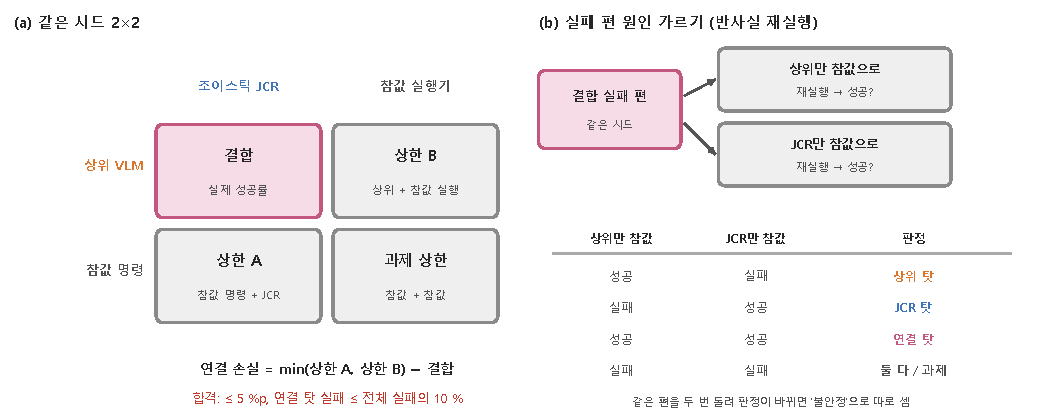
\includegraphics[width=\linewidth]{figures/f6_coupling_loss.pdf}
\caption{\textbf{연결 손실과 원인 분리.} (a) 같은 시드에서 \{상위, 참값 명령\} $\times$ \{JCR, 참값 실행기\} 네 칸을 돌린다. 참값은 시뮬 특권 정보로 계산한 명령·실행이다. (b) 결합 실패 편은 한쪽만 참값으로 바꿔 다시 돌려 원인을 가른다. 판정이 바뀌는 편은 `불안정'으로 따로 센다.}
\label{fig:closs}
\end{figure*}

같은 시드에서 네 칸의 성공률을 잰다(\cref{fig:closs}a). $S_{\text{결합}}$은 상위+JCR, $S_A$는 참값 명령+JCR, $S_B$는 상위+참값 실행기, $S_{\text{과제}}$는 참값+참값이다.
\begin{equation}
  \mathrm{CL} \;=\; \min(S_A,\ S_B) \;-\; S_{\text{결합}}.
\end{equation}
네 칸 모두 같은 코드 어댑터를 거친다 — 참값 명령도 어댑터가 JCR 명령(목적지·마스크·단계·허용·끌림 세기)으로 바꾼 뒤 준다. $S_A$와 $S_B$는 각 모듈이 완벽한 짝을 만났을 때의 상한이므로, 둘 중 낮은 쪽보다 결합이 더 낮은 만큼이 연결에서 샌 성능이다. 결합 실패 편은 한쪽만 참값으로 바꿔 재실행한다. 상위만 바꿔 성공하면 상위 탓, JCR만 바꿔 성공하면 JCR 탓, 어느 쪽을 바꿔도 성공하면 각자는 참값 짝과 되는데 둘이 함께 실패한 것이므로 연결 탓, 둘 다 실패하면 둘 다 또는 과제 탓으로 적는다(\cref{fig:closs}b). 같은 편을 두 번 돌려 판정이 바뀌면 `불안정'으로 따로 센다. 시뮬 물리는 매 편 시작에서 장면을 다시 만들어 같은 시드가 같은 궤적을 재생한다.

\paragraph{합격 기준.} $\mathrm{CL} \le 5$\,\%p, 그리고 연결 탓 실패 $\le$ 전체 실패의 10\,\%. 두 조건을 모두 넘어야 H-C를 지지한다고 본다.
